By selecting e$^{+}$e$^{-}$ pairs from the triggered events we're able to study basic distributions of pair production kinematics and in particular those related to our vertex performance. Pairs of opposite charge tracks, one in the top and one in the bottom half of the SVT, with larger than 400~MeV was selected. The pair production kinematics are relatively well reproduced given the alignment of the tracker; Fig.~\ref{fig:pair_kin} shows the invariant mass and ratio of electron momentum over the sum of electron and positron. 
\begin{figure}[ht]
%   \includegraphics[ width=0.4\textwidth]{test2012/vertexing/figures/h_invM_h_invM_dataMC_0016x0_oneclselgoodquadranttwotrksel}
   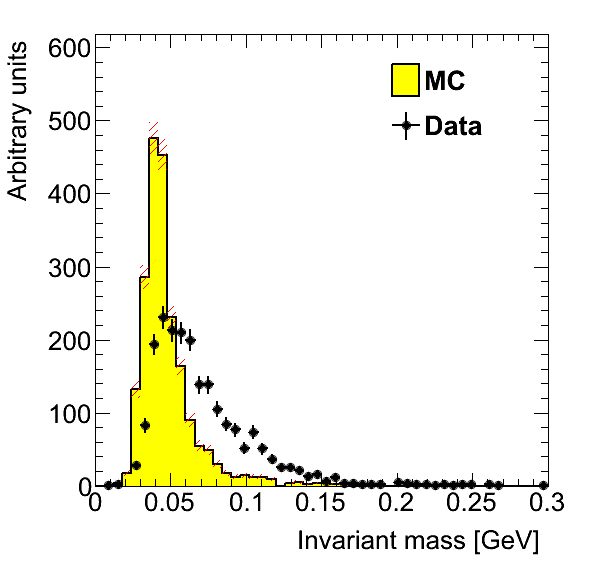
\includegraphics[scale=0.25]{test2012/vertexing/figures/h_invM_h_invM_dataMC_0016x0_twotrksel.png}
   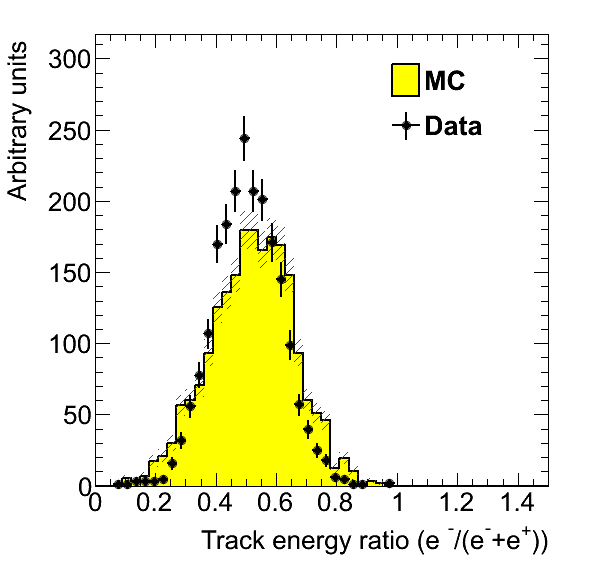
\includegraphics[scale=0.25]{test2012/vertexing/figures/h_ratioEsum_h_ratioEsum_dataMC_0016x0_twotrksel.png}
\caption{\small{The reconstructed invariant mass (left) and ratio of electron momentum over the momentum sum for pairs (right) of opposite charge tracks selected in the top and bottom half of the tracker.}}
\label{fig:pair_kin}
\end{figure}

As previously mentioned, the large distance to the converter and low statistics of the Test Run makes it hard 
to study the vertex resolution regime and tails of vertex distributions expected in the electron run. 
Nevertheless, we're able to compare the data in the Test Run with simulation to verify that our description 
of the multiple scattering is correct. 
Figure~\ref{fig:vtx_pos} shows the distance of closest approach of the momentum vectors extrapolated in the 
upstream direction from our analyzing magnet, taking into account the measured fringe field. 
 \begin{figure*}[t]
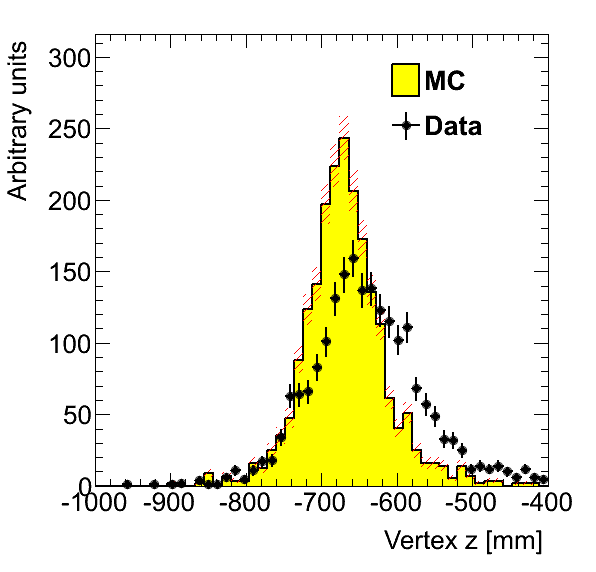
\includegraphics[ scale=0.25]{test2012/vertexing/figures/h_vtx_fr_x_h_vtx_x_dataMC_twotrksel.png}
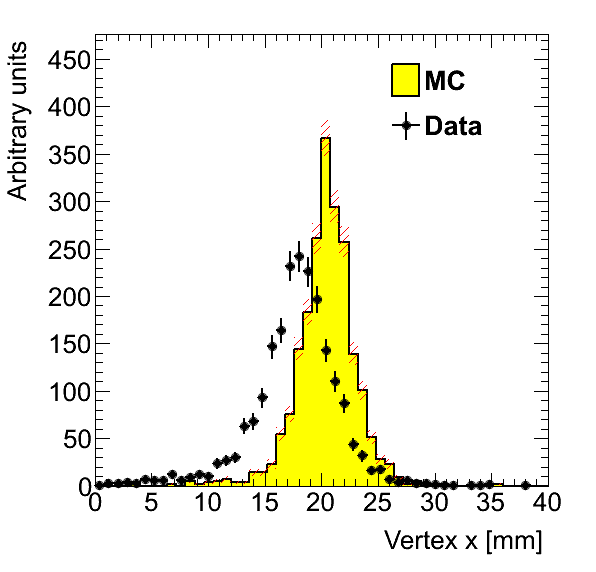
\includegraphics[ scale=0.25]{test2012/vertexing/figures/h_vtx_fr_y_h_vtx_y_dataMC_twotrksel.png}
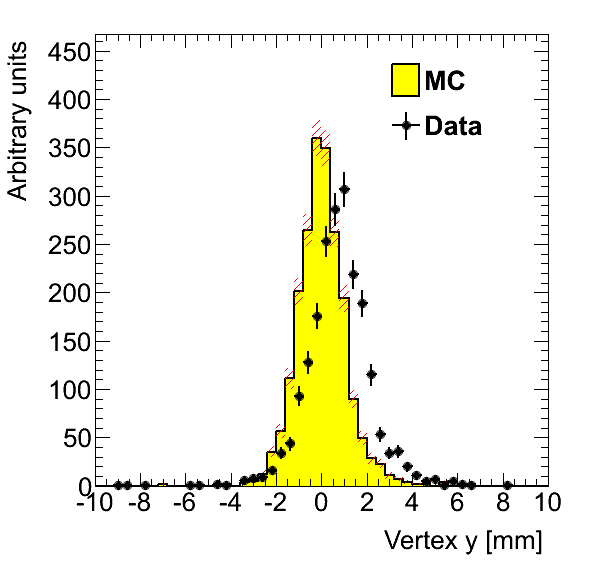
\includegraphics[ scale=0.25]{test2012/vertexing/figures/h_vtx_fr_z_h_vtx_z_dataMC_twotrksel.png}
\caption{\small{Vertex position represented by the distance of closest approach of the extrapolated momentum vectors upstream of the analyzing magnet. The overall shift from zero is due to a 30~mrad rotation of the SVT with respect to the beam line.}}\label{fig:vtx_pos}
\end{figure*}
While the tails of the vertex distribution in the physics running in an electron beam is 
in another regime the fact that the core is relatively well described provides confidence of the 
description of the multiple scattering which dominates the resolution, both in the Test Run and in 
electron beam running. 
